% Lecture 1: Foundations of Derivatives and Monotonicity (Beamer Presentation)
\documentclass[aspectratio=169]{beamer}
\usepackage{amsmath, amssymb, graphicx, tikz, pgfplots}
\pgfplotsset{compat=1.18}

\usetheme{Madrid}
\usecolortheme{default}

\title{Foundations of Derivatives and Monotonicity}
\subtitle{Lecture 1}
\author{}
\date{}

\begin{document}

\frame{\titlepage}

\begin{frame}{Plan}
\begin{enumerate}
\item \textbf{Function Limits} -- Intuition and $\varepsilon$-$\delta$ definition
\item \textbf{Derivative Definition} -- As a limit of difference quotient
\item \textbf{Monotonicity} -- Using derivatives to determine increase/decrease
\item \textbf{Derivative Rules} -- Sum, product, quotient rules
\item \textbf{Common Derivatives} -- Essential derivative formulas
\end{enumerate}
\end{frame}

\begin{frame}{Learning Objectives}
By the end of this lecture, you should be able to:
\begin{itemize}
\item Understand limits using the $\varepsilon$-$\delta$ definition
\item Define and compute derivatives from first principles
\item Identify whether a function is increasing or decreasing using its derivative
\item Apply differentiation rules efficiently
\item Recall and use common derivative formulas
\end{itemize}
\end{frame}

\section{Function Limits}

\begin{frame}{Intuitive Idea of a Limit}
\textbf{Question:} What value does $f(x)$ approach as $x$ gets closer to $a$?

\vspace{0.5cm}

We write: $\displaystyle \lim_{x \to a} f(x) = L$

\vspace{0.5cm}

This means: as $x$ approaches $a$, the function values $f(x)$ approach $L$.

\vspace{0.5cm}

\textbf{Key insight:} The limit describes behavior \textit{near} a point, not necessarily \textit{at} the point.
\end{frame}

\begin{frame}{Example: Computing a Limit}
\textbf{Example:}
\[
\lim_{x \to 2} \frac{x^2 - 4}{x - 2}
\]

If we substitute $x = 2$ directly, we get $\frac{0}{0}$, which is indeterminate.

\vspace{0.5cm}

However, we can simplify:
\[
\frac{x^2 - 4}{x - 2} = \frac{(x-2)(x+2)}{x-2} = x + 2, \quad x \neq 2
\]
Therefore,
\[
\lim_{x \to 2} \frac{x^2 - 4}{x - 2} = \lim_{x \to 2} (x+2) = 4
\]
\end{frame}

\begin{frame}{The $\varepsilon$-$\delta$ Definition of Limit}
\textbf{Formal Definition:} We say $\displaystyle \lim_{x \to a} f(x) = L$ if:

\vspace{0.3cm}

For every $\varepsilon > 0$, there exists a $\delta > 0$ such that whenever 
\[
0 < |x - a| < \delta \quad \Rightarrow \quad |f(x) - L| < \varepsilon
\]

\vspace{0.5cm}

\textbf{Interpretation:}
\begin{itemize}
\item $\varepsilon$ measures how close $f(x)$ is to $L$
\item $\delta$ measures how close $x$ is to $a$
\item No matter how small $\varepsilon$ is, we can find a $\delta$ that works
\end{itemize}
\end{frame}

\begin{frame}{Visualizing $\varepsilon$-$\delta$}
\begin{center}
\begin{tikzpicture}[scale=0.8]
\draw[->] (-0.5,0) -- (5,0) node[right] {$x$};
\draw[->] (0,-0.5) -- (0,4) node[above] {$y$};
\draw[blue, thick, domain=0.5:4.5] plot (\x, {0.5*\x + 1});
\draw[dashed] (2,0) node[below] {$a$} -- (2,2);
\draw[dashed] (0,2) node[left] {$L$} -- (2,2);
\draw[red, dashed] (0,1.5) node[left] {$L-\varepsilon$} -- (5,1.5);
\draw[red, dashed] (0,2.5) node[left] {$L+\varepsilon$} -- (5,2.5);
\draw[green!60!black, thick] (1.5,0) node[below] {$a-\delta$} -- (1.5,0.1);
\draw[green!60!black, thick] (2.5,0) node[below] {$a+\delta$} -- (2.5,0.1);
\fill[red] (2,2) circle (2pt);
\end{tikzpicture}
\end{center}
When $x$ is within $\delta$ of $a$, then $f(x)$ is within $\varepsilon$ of $L$.
\end{frame}

\begin{frame}{More Limit Examples}
\textbf{Example 1:} $\displaystyle \lim_{x \to 3} \frac{x^2 - 9}{x - 3}$

Factor: $\frac{(x-3)(x+3)}{x-3} = x+3$ for $x \neq 3$

Therefore: $\displaystyle \lim_{x \to 3} \frac{x^2 - 9}{x - 3} = 6$

\vspace{0.5cm}

\textbf{Example 2:} $\displaystyle \lim_{x \to 0} \frac{\sin x}{x} = 1$ (standard result)

\vspace{0.3cm}

These examples show that limits can be computed by algebraic simplification or known standard results.
\end{frame}

\section{Derivative Definition}

\begin{frame}{Motivation: The Slope Problem}
How do we find the slope of a curve at a single point?

\vspace{0.5cm}

For two points, the slope is:
\[
\text{slope} = \frac{f(x+h) - f(x)}{h}
\]

\vspace{0.5cm}

But what happens as the second point gets infinitely close to the first?

\vspace{0.3cm}

We take a \textbf{limit}!
\end{frame}

\begin{frame}{Definition of the Derivative}
The derivative of $f$ at $x$ is defined as:
\[
f'(x) = \lim_{h \to 0} \frac{f(x+h) - f(x)}{h}
\]

\vspace{0.5cm}

\textbf{Interpretation:}
\begin{itemize}
\item Instantaneous rate of change of $f$ at $x$
\item Slope of the tangent line to the graph of $f$ at point $(x, f(x))$
\end{itemize}
\end{frame}

\begin{frame}{Example: Derivative of $x^2$ from First Principles}
For $f(x) = x^2$:
\begin{align*}
f'(x) &= \lim_{h \to 0} \frac{(x+h)^2 - x^2}{h} \\
&= \lim_{h \to 0} \frac{x^2 + 2xh + h^2 - x^2}{h} \\
&= \lim_{h \to 0} \frac{2xh + h^2}{h} \\
&= \lim_{h \to 0} (2x + h) = 2x
\end{align*}

\vspace{0.3cm}
Therefore: $(x^2)' = 2x$
\end{frame}

\begin{frame}{Example: Derivative of $e^x$}
For $f(x) = e^x$:
\begin{align*}
f'(x) &= \lim_{h \to 0} \frac{e^{x+h} - e^x}{h} \\
&= \lim_{h \to 0} \frac{e^x \cdot e^h - e^x}{h} \\
&= e^x \lim_{h \to 0} \frac{e^h - 1}{h} \\
&= e^x \cdot 1 = e^x
\end{align*}

\vspace{0.3cm}
Therefore: $(e^x)' = e^x$

\vspace{0.2cm}
\small{(Using the standard result: $\displaystyle \lim_{h \to 0} \frac{e^h - 1}{h} = 1$)}
\end{frame}

\section{Monotonicity}

\begin{frame}{Monotonically Increasing and Decreasing Functions}
A function $f$ is said to be:
\begin{itemize}
\item \textbf{Monotonically increasing} on an interval if for all $x_1 < x_2$ in that interval, we have $f(x_1) < f(x_2)$
\item \textbf{Monotonically decreasing} on an interval if for all $x_1 < x_2$ in that interval, we have $f(x_1) > f(x_2)$
\end{itemize}

\vspace{0.5cm}

\textbf{Geometric interpretation:}
\begin{itemize}
\item Increasing: graph rises as we move left to right
\item Decreasing: graph falls as we move left to right
\end{itemize}
\end{frame}

\begin{frame}{Connection to Derivatives}
\textbf{Key Theorem:}
\[
f'(x) > 0 \Rightarrow f \text{ is increasing}, \quad f'(x) < 0 \Rightarrow f \text{ is decreasing}
\]

\vspace{0.5cm}

The derivative tells us whether the slope of the tangent line is positive (rising) or negative (falling).

\vspace{0.5cm}

\textbf{Why?} If $f'(x) > 0$, the function is going "uphill" at $x$.
\end{frame}

\begin{frame}{Example: Monotonicity of $f(x) = x^2$}
We computed $f'(x) = 2x$

\vspace{0.5cm}

\textbf{Analysis:}
\begin{itemize}
\item When $x < 0$: $f'(x) = 2x < 0$, so $f$ is decreasing
\item When $x > 0$: $f'(x) = 2x > 0$, so $f$ is increasing
\item At $x = 0$: $f'(x) = 0$ (critical point)
\end{itemize}

\vspace{0.5cm}

Conclusion: $f(x) = x^2$ decreases on $(-\infty, 0)$ and increases on $(0, \infty)$.
\end{frame}

\begin{frame}{Exercise: Monotonicity of $f(x) = x^3 - 3x$}
Determine where the function $f(x) = x^3 - 3x$ is increasing and where it is decreasing.

\vspace{0.3cm}

\textbf{Solution:}
\begin{align*}
f'(x) &= 3x^2 - 3 = 3(x^2 - 1) = 3(x-1)(x+1)
\end{align*}

Critical points: $x = -1$ and $x = 1$

\vspace{0.3cm}
Sign analysis:
\begin{itemize}
\item $(-\infty, -1)$: $f'(x) > 0$ (increasing)
\item $(-1, 1)$: $f'(x) < 0$ (decreasing)
\item $(1, \infty)$: $f'(x) > 0$ (increasing)
\end{itemize}
\end{frame}

\section{Derivative Rules}

\begin{frame}{Proof Outline: Sum Rule}
Using the definition of the derivative and linearity of limits:
\[
(f+g)'(x)=\lim_{h\to 0} \frac{f(x+h)-f(x)}{h}+\lim_{h\to 0} \frac{g(x+h)-g(x)}{h}=f'(x)+g'(x)
\]
\end{frame}

\begin{frame}{Proof Outline: Product Rule}
Start from the difference quotient and add--subtract $f(x)g(x+h)$:
\begin{align*}
(fg)'(x)
&= \lim_{h\to 0} \frac{f(x+h)g(x+h)-f(x)g(x)}{h} \\
&= \lim_{h\to 0} \frac{f(x+h)g(x+h)-f(x)g(x+h)+f(x)g(x+h)-f(x)g(x)}{h} \\
&= \lim_{h\to 0} \left[ \frac{f(x+h)-f(x)}{h}\cdot g(x+h) + f(x)\cdot\frac{g(x+h)-g(x)}{h} \right] \\
&= f'(x)g(x)+f(x)g'(x)
\end{align*}
\end{frame}

\begin{frame}{Proof Outline: Quotient Rule}
Write $\dfrac{f}{g}=f\cdot g^{-1}$ and use the product rule with $(g^{-1})'=-g'/g^2$:
\[
\left(\frac{f}{g}\right)'=f'g^{-1}+f\cdot(g^{-1})' = \frac{f'}{g}-f\cdot\frac{g'}{g^2}=\frac{f'g-fg'}{g^2}
\]
\end{frame}

\begin{frame}{Sum Rule}
\[
(f + g)' = f' + g'
\]

\vspace{0.5cm}
\textbf{Example:} If $f(x) = x^2$ and $g(x) = e^x$, then 
\[
(f + g)' = 2x + e^x
\]
\end{frame}

\begin{frame}{Product Rule}
\[
(fg)' = f'g + fg'
\]

\vspace{0.5cm}
\textbf{Example:} $f(x) = x^2 e^x$
\begin{align*}
f'(x) &= 2x e^x + x^2 e^x = e^x(2x + x^2)
\end{align*}
\end{frame}

\begin{frame}{Quotient Rule}
\[
\left(\frac{f}{g}\right)' = \frac{f'g - fg'}{g^2}
\]

\vspace{0.5cm}
\textbf{Example:} $f(x) = \frac{\sin x}{x}$
\begin{align*}
f'(x) &= \frac{x\cos x - \sin x}{x^2}
\end{align*}
\end{frame}

\section{Common Derivatives}

\begin{frame}{Power Functions}
\textbf{Power Rule:}
\[
\frac{d}{dx} x^n = nx^{n-1}
\]

\vspace{0.5cm}

\textbf{Examples:}
\begin{align*}
\frac{d}{dx} x^3 &= 3x^2 \\
\frac{d}{dx} x^{1/2} &= \frac{1}{2}x^{-1/2} = \frac{1}{2\sqrt{x}} \\
\frac{d}{dx} \frac{1}{x} = \frac{d}{dx} x^{-1} &= -x^{-2} = -\frac{1}{x^2}
\end{align*}
\end{frame}

\begin{frame}{Exponential and Logarithmic Functions}
\begin{align*}
\frac{d}{dx} e^x &= e^x \\[0.3cm]
\frac{d}{dx} a^x &= a^x \ln a \quad (a > 0) \\[0.3cm]
\frac{d}{dx} \ln x &= \frac{1}{x} \\[0.3cm]
\frac{d}{dx} \log_a x &= \frac{1}{x \ln a}
\end{align*}
\end{frame}

\begin{frame}{Trigonometric Functions}
\begin{align*}
\frac{d}{dx} \sin x &= \cos x \\[0.3cm]
\frac{d}{dx} \cos x &= -\sin x \\[0.3cm]
\frac{d}{dx} \tan x &= \sec^2 x = \frac{1}{\cos^2 x} \\[0.3cm]
\frac{d}{dx} \cot x &= -\csc^2 x = -\frac{1}{\sin^2 x}
\end{align*}
\end{frame}

\begin{frame}{More Trigonometric Functions}
\begin{align*}
\frac{d}{dx} \sec x &= \sec x \tan x \\[0.3cm]
\frac{d}{dx} \csc x &= -\csc x \cot x
\end{align*}
\end{frame}

\begin{frame}{Inverse Trigonometric Functions}
\begin{align*}
\frac{d}{dx} \arcsin x &= \frac{1}{\sqrt{1-x^2}} \\[0.3cm]
\frac{d}{dx} \arccos x &= -\frac{1}{\sqrt{1-x^2}} \\[0.3cm]
\frac{d}{dx} \arctan x &= \frac{1}{1+x^2}
\end{align*}
\end{frame}

\begin{frame}{Constants and Linear Functions}
\begin{align*}
\frac{d}{dx} c &= 0 \quad \text{(constant)} \\[0.3cm]
\frac{d}{dx} cx &= c \\[0.3cm]
\frac{d}{dx} (mx + b) &= m
\end{align*}

\vspace{0.5cm}

\textbf{Remember:} The derivative of a constant is always zero!
\end{frame}

\section{Visual Examples}

\begin{frame}{Graph of $y=x^2$}
\begin{center}
\begin{tikzpicture}
\begin{axis}[width=0.6\textwidth, height=0.5\textwidth, xlabel={$x$}, ylabel={$y$}, title={$y=x^2$}]
\addplot[samples=200, domain=-3:3, blue, thick]{x^2};
\end{axis}
\end{tikzpicture}
\end{center}
\vspace{-0.2cm}
Decrease on $(-\infty,0)$ and increase on $(0,\infty)$.
\end{frame}

\begin{frame}{Graph of $y=e^x$}
\begin{center}
\begin{tikzpicture}
\begin{axis}[width=0.6\textwidth, height=0.5\textwidth, xlabel={$x$}, ylabel={$y$}, title={$y=e^x$}]
\addplot[samples=200, domain=-3:3, red, thick]{exp(x)};
\end{axis}
\end{tikzpicture}
\end{center}
\vspace{-0.2cm}
Note: $\frac{d}{dx}e^x=e^x>0$, so it is increasing everywhere.
\end{frame}

\begin{frame}{Graph of $y=x^3-3x$}
\begin{center}
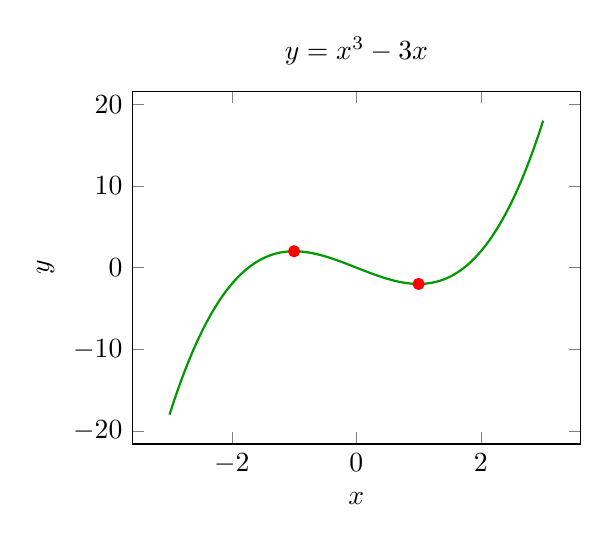
\begin{tikzpicture}
\begin{axis}[width=0.6\textwidth, height=0.5\textwidth, xlabel={$x$}, ylabel={$y$}, title={$y=x^3-3x$}]
\addplot[samples=300, domain=-3:3, green!60!black, thick]{x^3-3*x};
\addplot[mark=*, only marks, red] coordinates {(-1,2) (1,-2)}; % critical points
\end{axis}
\end{tikzpicture}
\end{center}
\vspace{-0.2cm}
Critical points at $x=\pm1$. Increasing on $(-\infty,-1)$ and $(1,\infty)$; decreasing on $(-1,1)$.
\end{frame}

\begin{frame}{Graph of $y=\frac{\sin x}{x}$ near 0}
\begin{center}
\begin{tikzpicture}
\begin{axis}[width=0.6\textwidth, height=0.5\textwidth, xlabel={$x$}, ylabel={$y$}, title={$y=\frac{\sin x}{x}$ near 0}, domain=-3.1:3.1]
\addplot[samples=600, domain=-3.1:-0.1, purple, thick]{sin(deg(x))/x};
\addplot[samples=600, domain=0.1:3.1, purple, thick]{sin(deg(x))/x};
\addplot[mark=*, only marks, red] coordinates {(0,1)}; % removable discontinuity
\end{axis}
\end{tikzpicture}
\end{center}
\vspace{-0.2cm}
The removable discontinuity is filled by $\lim_{x\to0} \frac{\sin x}{x}=1$.
\end{frame}

\section{Summary}

\begin{frame}{Summary}
\begin{enumerate}
\item \textbf{Limits:} Defined using $\varepsilon$-$\delta$; describes function behavior near a point
\item \textbf{Derivatives:} Defined as $f'(x) = \lim_{h \to 0} \frac{f(x+h) - f(x)}{h}$; measures instantaneous rate of change
\item \textbf{Monotonicity:} $f'(x) > 0$ means increasing; $f'(x) < 0$ means decreasing
\item \textbf{Rules:} Sum, product, and quotient rules for efficient differentiation
\item \textbf{Common Derivatives:} Power rule, exponential, logarithmic, trigonometric functions
\end{enumerate}
\end{frame}

\section{Homework}

\begin{frame}{Homework Problem 1}
Find intervals of increase/decrease for $f(x) = x^3 - 6x^2 + 9x$.
\end{frame}

\begin{frame}{Homework Problem 2}
Compute the following limits:
\begin{enumerate}
\item $\displaystyle \lim_{x \to 1} \frac{x^3 - 1}{x - 1}$
\item $\displaystyle \lim_{x \to 0} \frac{1 - \cos x}{x^2}$
\end{enumerate}
\end{frame}

\begin{frame}{Homework Problem 3}
Differentiate:
\begin{enumerate}
\item $f(x) = e^x + x^3$
\item $f(x) = x^2 e^x$
\item $f(x) = \frac{1}{x^2 + 1}$
\end{enumerate}
\end{frame}

\begin{frame}{}
\begin{center}
{\Huge Thank You!}

\vspace{1cm}

Questions?
\end{center}
\end{frame}

\end{document}
